\chapter{Auswertung und Diskussion}
\label{chap:evaluation}

Nachfolgende sollen nun die Ergebnisse der Migration der zwei Projekte von TeamShirts, die mit Hilfe des umgesetzten Flow-Transpilers durchgeführt wurde, dargelegt werden. Dabei wird einerseits die Erfüllung der Zielvorgaben aus Abschnitt~\ref{sec:goals}, andererseits die Einhaltung der technischen Anforderungen an den Transpiler aus Abschnitt~\ref{sec:requirements} beurteilt und kritisch diskutiert. Zunächst wird jedoch die Durchführung der Migration an sich beschrieben.

\section{Durchführung der Migration}

Bereits während der Entwicklungsphase des Flow-Transpilers wurde dieser immer wieder mit dem Quelltext der vorliegenden Projekte von TeamShirts erprobt, um dessen Praxistauglichkeit anhand einer realen Codebasis zu überprüfen. Nachdem der vollständige Funktionsumfang des Babel-Plugins hergestellt war, wurde zunächst das Projekt \textit{Components}, danach \textit{Helios} mit Hilfe des Flow-Übersetzers in TypeScript umgewandelt. Diese Reihenfolge wurde bewusst gewählt, weil Components einerseits keine Abhängigkeit zu anderen Projekten von TeamShirts besitzt, andererseits weniger Zeilen\footnote{Vgl. Abschnitt~\ref{sec:teamshirts-projects}} Code umfasst als Helios.

% components: 360 modules not found
Unmittelbar nach Ausführung des Transpilers wurden bei Components 195 neue Typfehler durch den TypeScript-Compiler festgestellt, die daraufhin manuell korrigiert werden mussten. Aufgrund der prinzipiellen Unterschiede der Typsysteme von Flow und Typescript, die im Grundlagenteil bereits ausgeführt wurden, war das Auftreten neuer Fehler zu erwarten. Wie beschrieben ist beispielsweise die Typinferenz und die Berechnung der Typkompatibilität (nominal versus strukturell) in TypeScript anders umgesetzt als bei Flow. In Abschnitt~\ref{goal:new-type-errors} wird dieser Aspekt näher beleuchtet und genauer beschrieben, welche Arten von Typfehlern neu aufgetreten sind. Gleichzeitig wird untersucht, ob die neu erkannten Typfehler tatsächlich bislang unentdeckte Programmfehler repräsentieren.

% Anwendung Transpiler
% Fixen von manuellen Fehlern
% optimierungen und decorator weil kacke

% Vorteile: Andere Projekte wie Helios, die Components verwenden, kriegen deren Typisierung "frei Haus".


\section{Bewertung der Ergebnisse hinsichtlich der Zielvorgabe}
\subsection{Erkennung weiterer Typ- und Programmfehler}
\label{goal:new-type-errors}

Der TypeScript-Compiler besitzt wie in Abschnitt~\ref{sec:typescript} beschrieben verschiedene Optionen, um die Striktheit der Typüberprüfungen zu erhöhen. Diese kann durch Setzen der Option \enquote{\code{strict}} angepasst werden, sodass daraufhin deutlich mehr Ausdrücke als Typfehler betrachtet werden.

% TODO: histogramme mit top 8 fehlern oder so strikt vs nicht-strikt
% TODO: erklärung: wo kommen diese fehler her? welche davon sind tatsächlich problematisch? welche nur bs von ts?
% TODO: ein paar beispiele für echte probleme

\subsection{Unterstützung externer Bibliotheken}

% TODO: vergleich flow-typed definitely typed
% TODO: 3 "schöne" bibs rauspicken (react, redux, lodash, datefns?) und libdefs vergleichen

\subsection{Performance der Typüberprüfungen}

% TODO: messungen (complete) für 4 geräte (tabelle reicht wohl)
% TODO: wenn ts multicore könnte, dann ...

\begin{figure}[tbp]
  \centering

  % GNUPLOT: LaTeX picture with Postscript
\begingroup
  \makeatletter
  \providecommand\color[2][]{%
    \GenericError{(gnuplot) \space\space\space\@spaces}{%
      Package color not loaded in conjunction with
      terminal option `colourtext'%
    }{See the gnuplot documentation for explanation.%
    }{Either use 'blacktext' in gnuplot or load the package
      color.sty in LaTeX.}%
    \renewcommand\color[2][]{}%
  }%
  \providecommand\includegraphics[2][]{%
    \GenericError{(gnuplot) \space\space\space\@spaces}{%
      Package graphicx or graphics not loaded%
    }{See the gnuplot documentation for explanation.%
    }{The gnuplot epslatex terminal needs graphicx.sty or graphics.sty.}%
    \renewcommand\includegraphics[2][]{}%
  }%
  \providecommand\rotatebox[2]{#2}%
  \@ifundefined{ifGPcolor}{%
    \newif\ifGPcolor
    \GPcolortrue
  }{}%
  \@ifundefined{ifGPblacktext}{%
    \newif\ifGPblacktext
    \GPblacktexttrue
  }{}%
  % define a \g@addto@macro without @ in the name:
  \let\gplgaddtomacro\g@addto@macro
  % define empty templates for all commands taking text:
  \gdef\gplbacktext{}%
  \gdef\gplfronttext{}%
  \makeatother
  \ifGPblacktext
    % no textcolor at all
    \def\colorrgb#1{}%
    \def\colorgray#1{}%
  \else
    % gray or color?
    \ifGPcolor
      \def\colorrgb#1{\color[rgb]{#1}}%
      \def\colorgray#1{\color[gray]{#1}}%
      \expandafter\def\csname LTw\endcsname{\color{white}}%
      \expandafter\def\csname LTb\endcsname{\color{black}}%
      \expandafter\def\csname LTa\endcsname{\color{black}}%
      \expandafter\def\csname LT0\endcsname{\color[rgb]{1,0,0}}%
      \expandafter\def\csname LT1\endcsname{\color[rgb]{0,1,0}}%
      \expandafter\def\csname LT2\endcsname{\color[rgb]{0,0,1}}%
      \expandafter\def\csname LT3\endcsname{\color[rgb]{1,0,1}}%
      \expandafter\def\csname LT4\endcsname{\color[rgb]{0,1,1}}%
      \expandafter\def\csname LT5\endcsname{\color[rgb]{1,1,0}}%
      \expandafter\def\csname LT6\endcsname{\color[rgb]{0,0,0}}%
      \expandafter\def\csname LT7\endcsname{\color[rgb]{1,0.3,0}}%
      \expandafter\def\csname LT8\endcsname{\color[rgb]{0.5,0.5,0.5}}%
    \else
      % gray
      \def\colorrgb#1{\color{black}}%
      \def\colorgray#1{\color[gray]{#1}}%
      \expandafter\def\csname LTw\endcsname{\color{white}}%
      \expandafter\def\csname LTb\endcsname{\color{black}}%
      \expandafter\def\csname LTa\endcsname{\color{black}}%
      \expandafter\def\csname LT0\endcsname{\color{black}}%
      \expandafter\def\csname LT1\endcsname{\color{black}}%
      \expandafter\def\csname LT2\endcsname{\color{black}}%
      \expandafter\def\csname LT3\endcsname{\color{black}}%
      \expandafter\def\csname LT4\endcsname{\color{black}}%
      \expandafter\def\csname LT5\endcsname{\color{black}}%
      \expandafter\def\csname LT6\endcsname{\color{black}}%
      \expandafter\def\csname LT7\endcsname{\color{black}}%
      \expandafter\def\csname LT8\endcsname{\color{black}}%
    \fi
  \fi
    \setlength{\unitlength}{0.0500bp}%
    \ifx\gptboxheight\undefined%
      \newlength{\gptboxheight}%
      \newlength{\gptboxwidth}%
      \newsavebox{\gptboxtext}%
    \fi%
    \setlength{\fboxrule}{0.5pt}%
    \setlength{\fboxsep}{1pt}%
\begin{picture}(7360.00,4520.00)%
    \gplgaddtomacro\gplbacktext{%
      \csname LTb\endcsname%%
      \put(596,652){\makebox(0,0)[r]{\strut{}$3$}}%
      \csname LTb\endcsname%%
      \put(596,1107){\makebox(0,0)[r]{\strut{}$4$}}%
      \csname LTb\endcsname%%
      \put(596,1563){\makebox(0,0)[r]{\strut{}$5$}}%
      \csname LTb\endcsname%%
      \put(596,2018){\makebox(0,0)[r]{\strut{}$6$}}%
      \csname LTb\endcsname%%
      \put(596,2474){\makebox(0,0)[r]{\strut{}$7$}}%
      \csname LTb\endcsname%%
      \put(596,2929){\makebox(0,0)[r]{\strut{}$8$}}%
      \csname LTb\endcsname%%
      \put(596,3384){\makebox(0,0)[r]{\strut{}$9$}}%
      \csname LTb\endcsname%%
      \put(596,3840){\makebox(0,0)[r]{\strut{}$10$}}%
      \csname LTb\endcsname%%
      \put(596,4295){\makebox(0,0)[r]{\strut{}$11$}}%
      \csname LTb\endcsname%%
      \put(1410,448){\makebox(0,0){\strut{}1}}%
      \csname LTb\endcsname%%
      \put(2111,448){\makebox(0,0){\strut{}2}}%
      \csname LTb\endcsname%%
      \put(2813,448){\makebox(0,0){\strut{}3}}%
      \csname LTb\endcsname%%
      \put(3515,448){\makebox(0,0){\strut{}4}}%
      \csname LTb\endcsname%%
      \put(4216,448){\makebox(0,0){\strut{}5}}%
      \csname LTb\endcsname%%
      \put(4918,448){\makebox(0,0){\strut{}6}}%
      \csname LTb\endcsname%%
      \put(5620,448){\makebox(0,0){\strut{}7}}%
      \csname LTb\endcsname%%
      \put(6321,448){\makebox(0,0){\strut{}8}}%
    }%
    \gplgaddtomacro\gplfronttext{%
      \csname LTb\endcsname%%
      \put(158,2473){\rotatebox{-270}{\makebox(0,0){\strut{}\small durchschnittliche Laufzeit in s}}}%
      \csname LTb\endcsname%%
      \put(3865,142){\makebox(0,0){\strut{}\small Anzahl eingesetzter Prozessorkerne}}%
      \csname LTb\endcsname%%
      \put(3865,3989){\makebox(0,0){\strut{}\small\bfseries Components}}%
      \csname LTb\endcsname%%
      \put(6158,4010){\makebox(0,0)[r]{\strut{}\small Flow}}%
      \csname LTb\endcsname%%
      \put(6158,3806){\makebox(0,0)[r]{\strut{}\small TypeScript}}%
    }%
    \gplbacktext
    \put(0,0){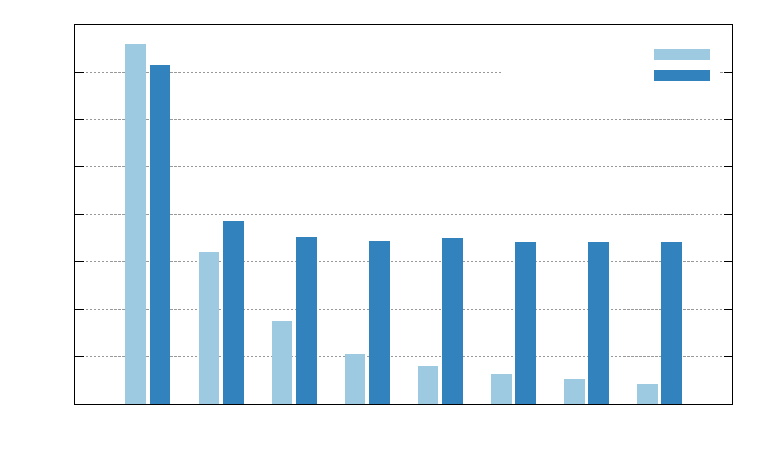
\includegraphics{../data/plots/complete/components-plot}}%
    \gplfronttext
  \end{picture}%
\endgroup


  \vspace{.5\baselineskip}

  % GNUPLOT: LaTeX picture with Postscript
\begingroup
  \makeatletter
  \providecommand\color[2][]{%
    \GenericError{(gnuplot) \space\space\space\@spaces}{%
      Package color not loaded in conjunction with
      terminal option `colourtext'%
    }{See the gnuplot documentation for explanation.%
    }{Either use 'blacktext' in gnuplot or load the package
      color.sty in LaTeX.}%
    \renewcommand\color[2][]{}%
  }%
  \providecommand\includegraphics[2][]{%
    \GenericError{(gnuplot) \space\space\space\@spaces}{%
      Package graphicx or graphics not loaded%
    }{See the gnuplot documentation for explanation.%
    }{The gnuplot epslatex terminal needs graphicx.sty or graphics.sty.}%
    \renewcommand\includegraphics[2][]{}%
  }%
  \providecommand\rotatebox[2]{#2}%
  \@ifundefined{ifGPcolor}{%
    \newif\ifGPcolor
    \GPcolortrue
  }{}%
  \@ifundefined{ifGPblacktext}{%
    \newif\ifGPblacktext
    \GPblacktexttrue
  }{}%
  % define a \g@addto@macro without @ in the name:
  \let\gplgaddtomacro\g@addto@macro
  % define empty templates for all commands taking text:
  \gdef\gplbacktext{}%
  \gdef\gplfronttext{}%
  \makeatother
  \ifGPblacktext
    % no textcolor at all
    \def\colorrgb#1{}%
    \def\colorgray#1{}%
  \else
    % gray or color?
    \ifGPcolor
      \def\colorrgb#1{\color[rgb]{#1}}%
      \def\colorgray#1{\color[gray]{#1}}%
      \expandafter\def\csname LTw\endcsname{\color{white}}%
      \expandafter\def\csname LTb\endcsname{\color{black}}%
      \expandafter\def\csname LTa\endcsname{\color{black}}%
      \expandafter\def\csname LT0\endcsname{\color[rgb]{1,0,0}}%
      \expandafter\def\csname LT1\endcsname{\color[rgb]{0,1,0}}%
      \expandafter\def\csname LT2\endcsname{\color[rgb]{0,0,1}}%
      \expandafter\def\csname LT3\endcsname{\color[rgb]{1,0,1}}%
      \expandafter\def\csname LT4\endcsname{\color[rgb]{0,1,1}}%
      \expandafter\def\csname LT5\endcsname{\color[rgb]{1,1,0}}%
      \expandafter\def\csname LT6\endcsname{\color[rgb]{0,0,0}}%
      \expandafter\def\csname LT7\endcsname{\color[rgb]{1,0.3,0}}%
      \expandafter\def\csname LT8\endcsname{\color[rgb]{0.5,0.5,0.5}}%
    \else
      % gray
      \def\colorrgb#1{\color{black}}%
      \def\colorgray#1{\color[gray]{#1}}%
      \expandafter\def\csname LTw\endcsname{\color{white}}%
      \expandafter\def\csname LTb\endcsname{\color{black}}%
      \expandafter\def\csname LTa\endcsname{\color{black}}%
      \expandafter\def\csname LT0\endcsname{\color{black}}%
      \expandafter\def\csname LT1\endcsname{\color{black}}%
      \expandafter\def\csname LT2\endcsname{\color{black}}%
      \expandafter\def\csname LT3\endcsname{\color{black}}%
      \expandafter\def\csname LT4\endcsname{\color{black}}%
      \expandafter\def\csname LT5\endcsname{\color{black}}%
      \expandafter\def\csname LT6\endcsname{\color{black}}%
      \expandafter\def\csname LT7\endcsname{\color{black}}%
      \expandafter\def\csname LT8\endcsname{\color{black}}%
    \fi
  \fi
    \setlength{\unitlength}{0.0500bp}%
    \ifx\gptboxheight\undefined%
      \newlength{\gptboxheight}%
      \newlength{\gptboxwidth}%
      \newsavebox{\gptboxtext}%
    \fi%
    \setlength{\fboxrule}{0.5pt}%
    \setlength{\fboxsep}{1pt}%
\begin{picture}(7360.00,4520.00)%
    \gplgaddtomacro\gplbacktext{%
      \csname LTb\endcsname%%
      \put(596,652){\makebox(0,0)[r]{\strut{}$4$}}%
      \csname LTb\endcsname%%
      \put(596,1172){\makebox(0,0)[r]{\strut{}$6$}}%
      \csname LTb\endcsname%%
      \put(596,1693){\makebox(0,0)[r]{\strut{}$8$}}%
      \csname LTb\endcsname%%
      \put(596,2213){\makebox(0,0)[r]{\strut{}$10$}}%
      \csname LTb\endcsname%%
      \put(596,2734){\makebox(0,0)[r]{\strut{}$12$}}%
      \csname LTb\endcsname%%
      \put(596,3254){\makebox(0,0)[r]{\strut{}$14$}}%
      \csname LTb\endcsname%%
      \put(596,3775){\makebox(0,0)[r]{\strut{}$16$}}%
      \csname LTb\endcsname%%
      \put(596,4295){\makebox(0,0)[r]{\strut{}$18$}}%
      \csname LTb\endcsname%%
      \put(1410,448){\makebox(0,0){\strut{}1}}%
      \csname LTb\endcsname%%
      \put(2111,448){\makebox(0,0){\strut{}2}}%
      \csname LTb\endcsname%%
      \put(2813,448){\makebox(0,0){\strut{}3}}%
      \csname LTb\endcsname%%
      \put(3515,448){\makebox(0,0){\strut{}4}}%
      \csname LTb\endcsname%%
      \put(4216,448){\makebox(0,0){\strut{}5}}%
      \csname LTb\endcsname%%
      \put(4918,448){\makebox(0,0){\strut{}6}}%
      \csname LTb\endcsname%%
      \put(5620,448){\makebox(0,0){\strut{}7}}%
      \csname LTb\endcsname%%
      \put(6321,448){\makebox(0,0){\strut{}8}}%
    }%
    \gplgaddtomacro\gplfronttext{%
      \csname LTb\endcsname%%
      \put(158,2473){\rotatebox{-270}{\makebox(0,0){\strut{}\small durchschnittliche Laufzeit in s}}}%
      \csname LTb\endcsname%%
      \put(3865,142){\makebox(0,0){\strut{}\small Anzahl eingesetzter Prozessorkerne}}%
      \csname LTb\endcsname%%
      \put(3865,3989){\makebox(0,0){\strut{}\small\bfseries Helios}}%
      \csname LTb\endcsname%%
      \put(6158,4010){\makebox(0,0)[r]{\strut{}\small Flow}}%
      \csname LTb\endcsname%%
      \put(6158,3806){\makebox(0,0)[r]{\strut{}\small TypeScript}}%
    }%
    \gplbacktext
    \put(0,0){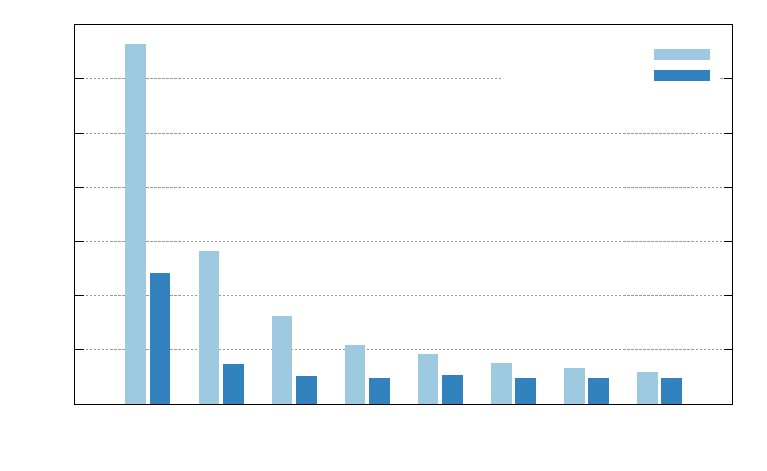
\includegraphics{../data/plots/complete/helios-plot}}%
    \gplfronttext
  \end{picture}%
\endgroup

  \vspace{.5\baselineskip}
  \caption[Einfluss der zur Verfügung stehenden Rechenkerne auf durchschnittliche Laufzeit der Typüberprüfung von Flow und TypeScript]{
    Einfluss der zur Verfügung stehenden Rechenkerne auf durchschnittliche Laufzeit der Typüberprüfung von Flow und TypeScript der Projekte \textit{Components} und \textit{Helios}.
  }

  \vspace{\baselineskip}
  \caption*{
    \small
    Jeweils 100 Messwerte, bestes und schlechtestes Dezil verworfen.\\
    Flow v0.96, TypeScript v3.5.\\
    Intel Core i7-6700 CPU mit 3,4~GHz.
  }
\end{figure}


\subsection{Zukunftssicherheit und Transparenz der Technologie}

% TODO: artikel: what we've been up to
% TODO: roadmap
% TODO: evtl berechnen wie lang issues im schnitt offen bleiben?


\section{Erfüllung der technischen Anforderungen}
\subsection{Äquivalente und vollständige Übersetzung der Flow-Typen}
\label{sec:interpretation:equivalent-translation}

\subsubsection{Äquivalenz der Übersetzungen}

Als erste und wichtigste technische Anforderung an den Transpiler wurde die äquivalente und vollständige Übersetzung der gesamten Flow-Syntax nach TypeScript definiert. Die äquivalenten TypeScript-Ausdrücke der verschiedenen Flow-Typen konnten dabei mehrheitlich einfach gefunden werden, weil TypeScript einen sehr ähnlichen Funktionsumfang wie Flow besitzt und sich oftmals nur die Schlüsselwörter unterscheiden\footnote{Vgl. Übersetzungstabellen in Abschnitt~\ref{sec:flow-transpilation}.}. Kompliziertere, nicht offensichtliche Transformationen wurden experimentell ermittelt.

Für einige, wenige Typen existiert keine absolut bedeutungsgleiche Übersetzung, weil TypeScript manche der Funktionen von Flow nicht unterstützt. Infolgedessen kommt es hier bei der Transpilierung zwingend zu einem Verlust von Typinformation, was in neuen Typfehlern resultieren kann. Die inkorrekte Transformation derartiger Typen wird gemäß Anforderung~\ref{sec:requirement:completeness} akzeptiert, jedoch muss der Benutzer bei Auftreten eines solchen Falls gewarnt werden. Quelltext~\ref{code:transpiler-warnings} zeigt wie eine solche Warnung aufgebaut ist. Dabei wird einerseits die genaue Position des verursachenden Flow-Typs im Quelltext angegeben, andererseits wird der Benutzer über die Hintergründe der Warnung durch einen Link informiert.

\begin{lstlisting}[
  label={code:transpiler-warnings},
  caption={Ausgabe von Warnungen bei Autreten nicht äquivalent übersetzbarer Flow-Typen.},
  emph={Warning},
]
Transpiling example.js...

  1 | // @flow
> 2 | const existentialType: * = String(2 * 3);
    |                       ^
  Warning: Flow's Existential Type (*) is not expressible in TypeScript.
           It will be replaced with 'any'.
           See https://github.com/Microsoft/TypeScript/issues/14466.
\end{lstlisting}

Nachfolgend wird dargelegt, welche der Funktionen von Flow nicht absolut korrekt übersetzt werden können und wie dies jeweils innerhalb des Transpilers gehandhabt wird.

\begin{itemize}
  \item {\libertineSB{Existential type}}\\*
    In TypeScript existiert kein Typ, der Flows \type{Existential type} entspricht~\autocite{TS:GITHUB:NO_EXISTENTIAL_TYPE}. Wie Quelltext~\ref{code:transpiler-warnings} bereits exemplarisch andeutet, wird dieser Typs deswegen durch den Typ \type{any} ersetzt. Weil \type{any} Supertyp jeden Typs ist, geht damit Typinformation verloren, sofern Flow zuvor einen konkreteren Typ inferieren konnte. Jedoch gibt die Dokumentation von Flow an, dass der \type{Existential type} oftmals tatsächlich äquivalent zu \type{any} ist~\autocite{FLOW:LINT_RULE_REFERENCE}.
  \medbreak
  \item {\libertineSB{Index-Signaturen in Objekttypen}}\\*
    Durch eckige Klammern kann in Objekttypen ein Index, also die Abbildung eines Typs von Namen auf Werte eines anderen Typs, angegeben werden\footnote{Vgl. Tabelle~\ref{tab:flow-base-types}.}. Flow unterstützt hierbei jeden beliebigen Typ für die Attributnamen, TypeScript hingegen nur \code{string} und \code{number}~\autocite{TS:HANDBOOK:INTERFACES}. Deshalb entfernt der Transpiler Index-Signaturen, die von diesen erlaubten Typen abweichen, und fügt stattdessen jeweils eine Signatur für \code{string} und \code{number} ein, um die größtmögliche Menge von Schlüsseltypen zu gewährleisten.
  \medbreak
  \item {\libertineSB{Opaque type}}\\*
    Auch opake Typen werden durch TypeScript nicht unterstützt~\autocite{TS:GITHUB:NO_OPAQUE_TYPE}. Infolgedessen wird dieser Typ bei der Übersetzung durch ein Typalias, das auf den gleichen Typ verweist, ersetzt.
  \medbreak
  \item {\libertineSB{Rückgabewert von Konstruktoren}}\\*
    Flow ermöglicht es den Rückgabewert von Konstruktorfunktionen explizit anzugeben. Dies ist in TypeScript bewusst verboten, weil es im Allgemeinen als schlechter Programmierstil erachtet wird, wenn ein Konstruktor etwas anderes als eine Klasseninstanz zurückliefert~\autocite{TS:GITHUB:CONSTRUCTOR_RETURN_TYPE}. Ein solcher Rückgabewert wird deswegen durch den Transpiler entfernt, damit keine fehlerhafte TypeScript-Syntax entsteht.
  \medbreak
  \item {\libertineSB{Varianz}}\\*
    Ein letzter Aspekt von Flow, der in TypeScript in einigen Fällen nicht abbildbar ist, ist die Varianz von Typen. Weil die Syntax von TypeScript nur Kovarianz (Schlüsselwort \code{readonly}) unterstützt, werden die Varianz-Signaturen von Flow für alle anderen Fälle verworfen. Dies beinhaltet neben Objektattributen beispielsweise auch Typparameter, die in Flow entsprechend markiert werden können.
\end{itemize}

\subsubsection{Vollständigkeit der Transformationen}

Wie bereits in Abschnitt~\ref{sec:requirement:completeness} ausgeführt ist der vollständige Funktionsumfang der Implementierung durch die Spezifikation des Parsers~\autocite{BABEL:PARSER_SPEC} von Babel präzise definiert, weil das Dokument festlegt, welche Knoten des abstrakten Syntaxbaums Flow-Syntax darstellen. Sofern sämtliche dieser Elemente korrekt in ihr TypeScript-Gegenstück transformiert werden, so ist die Vollständigkeit erreicht. Dies setzt vorraus, dass der abstrakte Syntaxbaum von Babel tatsächlich jegliche Flow-Syntax abbildet. Es konnte kein Beleg gefunden werden, der diese Annahme widerlegt.
Ein weitere Aspekt, der zur Erzielung einer vollständigen Umsetzung beiträgt, ist die Typisierung von Babel, da diese beispielsweise einen Vereinigungstyp \code{Flow} bereitstellt, der alle Knotentypen von Flow umfasst~\autocite{BABEL:TYPES}. Auf diese Weise kann statisch überprüft werden, ob das Babel-Plugin alle Elemente dieser Vereinigungsmenge verarbeitet. Sollten nicht alle Fälle behandelt werden, so kann dies durch eine Typverletzung offen gelegt werden\footnote{Vgl. beispielsweise zentrale Flow-Umwandlungsfunktion in Quelltext~\ref{code:convert-flow-type}. Die \code{switch}-Anweisung verarbeitet ausnahmslos alle Elemente des Typs \type{FlowType}. Dies kann statisch garantiert werden.}.

Die Korrektheit der Transformationen wird durch den in Abschnitt~\ref{sec:tdd} beschriebenen Ansatz der testgetriebenen Entwicklung gewährleistet. In der Dokumentation von Flow~\autocite{FLOW:TYPE_ANNOTATIONS} wird die Syntax aller Sprachkonstrukte beschrieben, sodass bekannt ist, welche Typen prinzipiell möglich sind. Durch Anlegen von Fixture-Dateien kann damit die korrekte Übersetzung sämtlicher Flow-Funktionen umfangreich getestet werden. Wie ausgeführt wurden insgesamt \numberOfTests Testfälle angelegt, um alle Basis- und Hilfstypen sowie Typdeklarationen zu überprüfen. Durch eine hohe Testabdeckung von 93\% wird darüber hinaus sicher gestellt, dass die verschiedenen Programmverzweigungen des Transpilers tatsächlich die angestrebte Funktionalität umsetzen.

% Insgesamt kann die Anforderung der äquivalenten und vollständigen Übersetzung aller Flow-Typen somit als erfüllt betrachtet werden.

\subsubsection{Vergleich mit konkurrierenden Transpilern}

Die zwei betrachteten Aspekte der Äquivalenz und Vollständigkeit der Transformationen sollen auch für die zwei konkurrierenden Ansätze von \textit{Kikura}~\autocite{KIKURA:FLOW_TO_TS} und der \textit{Khan Academy}~\autocite{KHAN:FLOW_TO_TS} betrachtet werden, um das erzielte Ergebnis einzuordnen.

TODO kiikurage hat bugs


\subsection{Semantisch äquivalente Transpilierung des Quelltexts}

Der Transpiler darf die Semantik des ursprünglichen JavaScript-Programms durch die Übersetzung nicht verändern, damit keine neuen Programmfehler in den Quelltext eingeschleust werden. Die Überprüfung der semantisch korrekten Übersetzung der Flow-Typen wurde bereits im vorherigen Abschnitt behandelt. Weil die statische Typisierung vor der Auslieferung vollständig entfernt wird, hat diese aber ohnehin keinen Einfluss auf die Laufzeit-Semantik des Programms, sofern deren Transformation fehlerfrei, ohne Nebenwirkung umgesetzt wurde. Ein Aspekt des umgesetzten Transcompilers, der zu abweichender Semantik führen könnte sind die in Abschnitt~\ref{sec:optimizations} beschriebenen optionalen Optimierungen der Ausgabe. Durch die Option \enquote{\code{replace-decorators}} werden beispielsweise Dekoratoren in bedeutungsgleiche verschachtelte Funktionsaufrufe umgewandelt.

Ein formaler Beweis der semantischen Äquivalenz ist aufgrund des Umfangs der zwei migrierten Projekte nicht durchführbar. Jedoch kann durch Betrachtung der bestehenden Modultests die Beibehaltung der Programmwirkung nach der Übersetzung zumindest approximativ verifiziert werden. Kritisch anzumerken ist, dass dieser Ansatz nur bei einer entsprechend hohen Testabdeckung aussagekräftig ist. Während diese bei Components bei 90,5\% liegt, wird bei Helios nur ein Anteil von 18,0\% erreicht. Nachdem alle nicht-strikten Typfehler in beiden Projekten korrigiert waren, wurden daraufhin die Modultests beider Projekte ausgeführt. Keiner der 373 Tests von Components und 326 Tests von Helios schlug dabei fehl, sodass die semantisch korrekten Überführung des ursprünglichen Quelltexts nach TypeScript wahrscheinlich ist.
Bei der praktischen Erprobung der zwei Projekte wurde allerdings in vier Fällen ein fehlerhaftes Verhalten der Webanwendung festgestellt. Jedoch konnte jedes dieser Probleme auf eine fehlerhafte händische Korrektur neuer Typfehler zurückgeführt werden.

\subsection{Unterstützung aktueller und vorläufiger JavaScript- sowie JSX-Syntax}

Die Anforderung aktuelle und vorläufige JavaScript- sowie JSX-Syntax zu unterstützen war eines der grundlegenden Kriterien anhand derer in Abschnitt~\ref{sec:js-transpilers} verschiedene Parser, Codegeneratoren und Transpiler bezüglich ihrer Eignung als Basis für die Umsetzung des Flow-Transpilers verglichen wurden. Wie dort bereits ausgeführt, ist der Babel nach Kenntnisstand des Autors das einzige Werkzeug, dass sowohl jegliche aktuelle, als auch vorläufige JavaScript-Syntax einlesen und verarbeiten kann. Ermöglicht wird dies durch eine Vielzahl von Plugins, welche die Verarbeitung von Flow, JSX und der in

% TODO: geht weil babel proposals, es2019 und jsx unterstützt

\subsection{Verarbeitung gesamter Projektverzeichnisse}

Wie in Abschnitt~\ref{sec:cli-program} bereits ausführlich dargelegt, wurde der Transpiler um ein Kommandozeilenprogramm (\textit{Reflow}) erweitert, um die Verarbeitung gesamter Verzeichnisse zu realisieren. Die Anwendung erwartet eine oder mehrere Dateien bzw. Verzeichnisse als Argument und setzt daraufhin die Übersetzung dieser Eingaben mit Hilfe des Babel-Plugins um.
Durch die interne Verwendung der Bibliothek \textit{Glob}~\autocite{NPM:GLOB} können dabei beliebig komplexe Wildcard-Muster (\textit{glob patterns}) verarbeitet werden, um gewisse Datei- oder Verzeichnistypen ein- und auszuschließen. Die Glob-Notation ähnelt konzeptionell regulären Ausdrücken in einigen Aspekten, sodass auch kompliziertere Muster, wie beispielsweise die Negation von Ausdrücken oder die Angabe einer Gruppe von alternativen Werten, möglich sind~\autocite{MAN:GLOB}.

% TODO: Vergleich zu Khan und Kikura

Die in Abschnitt~\ref{sec:requirement:batch-processing} definierten Forderungen, dass einerseits Verzeichnisse rekursiv verarbeitet werden, andererseits die Menge der zu übersetzenden Dateien flexibel eingegrenzt werden können muss, wurden somit erfüllt.

\subsection{Beibehaltung der Quelltext-Formatierung}

Weil die originalgetreue Formatierung der Ausgabe (Anforderung~\ref{sec:requirement:format}) bei Verwendung des Babel-Codegenerators, aus den dargelegten Gründen, nicht umsetzbar ist, wurde eine Formatierungsroutine auf Basis des Werkzeugs Prettier~\autocite{SOFTWARE:PRETTIER} implementiert\footnote{Vgl. Abschnitt~\ref{sec:formatting}}.
Mittels händischer Überprüfung des erzeugten TypeScript-Codes der zwei vorliegenden Projekte von TeamShirts, wurden inkorrekt formatierte Dateien ermittelt. Hierunter werden Dateien verstanden in denen Zeilen anders als im ursprünglichen Quelltext umgebrochen oder Leerzeilen und Kommentare falsch platziert werden. Sobald eine dieser Eigenschaften vorliegt, wird die Formatierung als fehlerhaft betrachtet. Wie Tabelle~\ref{tab:results-formatting} zeigt, gelingt diese leider nicht in allen Fällen. Während diese im Projekt Components bei 11 der 311 verarbeiteten JavaScript-Dateien (3,54\%) fehlgeschlagen ist, konnten bei Helios 21 der 353 Ausgabedateien nicht korrekt formatiert werden (5,95\%). Insgesamt ergibt sich somit eine Fehlerrate von 4,68\%.

\bigbreak
\begin{table}[tbh]
  \footnotesize
  \begin{tabu} to \textwidth {@{}lrrrrrr@{}}
    \midrule
    \libertineSB{Projekt} & \libertineSB{Dateien} & \libertineSB{falsch formatiert} & \libertineSB{rel. Anteil} & \libertineSB{Zeilen~$+$} & \libertineSB{Zeilen~$-$} & \libertineSB{Zeilen insg.} \\
    \midrule
    Components & 331 & 11 & 3,32\% & 2.564 & 2.417 & 32.240 \\
    Helios     & 353 & 21 & 5,95\% & 4.604 & 3.873 & 45.436 \\
    \midrule
    insgesamt  & 684 & 32 & 4,68\% & 7.168 & 6.290 & 77.675 \\
    \midrule
  \end{tabu}
  \caption{Ergebnisse der Formatierung der Ausgabequelltexte.}
  \label{tab:results-formatting}
\end{table}


\medbreak
Zur Feststellung der Ursachen der fehlerhaften Formatierung wurden die Verarbeitung der inkorrekt ausgegebenen Dateien untersucht. Weil das Verfahren zeilenbasiert arbeitet, ist die Konsistenz der Umbrüche für das Gelingen der Formatierung entscheidend, da es andernfalls zu einem Versatz der betrachteten Eingabe- und Ausgabgezeilen kommt. Die Betrachtung der Originaldateien, welche fehlerhaft formatiert wurden, hat gezeigt, dass dies in Folge von bestimmten, eher selten vorkommenden Quelltext-Formatierung auftritt. Nachfolgend soll das Problem anhand eines Beispiel für einen solchen Fall veranschaulicht werden:

\begin{lstlisting}[
  label={code:wrong-formatting:flow},
  caption={Beispiel für Formatierung des Original-Quelltexts, die falsch in die Ausgabe übernommen wird.}
]
if (
  a &&
  b &&    // Kommentar, der Zweck von 'b' beschreibt
  c === 0 // Kommentar, der Zweck von 'c' beschreibt
) {
  // ...
}
\end{lstlisting}

Der boolesche Ausdruck, der als Bedingung der Verzweigung in Zeile~1 dient, wird mehrmals umgebrochen, sodass der Zweck der einzelnen Elemente durch einen Zeilenkommentar erläutert werden kann. Der umgesetzte Flow-Transpiler ignoriert Kommentare der Eingabe bei Generierung der TypeScript-Ausgabe, weil Babel diese wie ausgeführt ohnehin falsch platzieren würde. Erst durch die Formatierungsroutine werden die Kommentare im Nachgang wieder eingefügt. Diese schlägt für das Beispiel fehl, weil der boolesche Ausdruck in der erzeugten Ausgabe aufgrund der entfernten Kommentare nicht mehr umgebrochen wird (vgl. Quelltext~\ref{code:wrong-formatting:ts}). Da der Zeilenumbruch in der Ein- und Ausgabe in diesem Fall somit inkonsistent ist, schlägt auch die Übertragung der Formatierung in allen nachfolgenden Zeilen fehl.

\begin{lstlisting}[
  % float,
  % floatplacement=H,
  label={code:wrong-formatting:ts},
  caption={Generierte TypeScript-Ausgabe der Eingabe in~\ref{code:wrong-formatting:flow} \emph{vor} Ausführung der Formatierungsroutine.}
]
if (foo && bar && baz === 0) {
  // ...
}
\end{lstlisting}

Wie die weitere Fehleranalyse gezeigt hat, ergibt sich bei der Auflistung der formalen Parameter von Funktionen die gleiche Problematik, wenn diese analog zum Beispiel umgebrochen werden. Zur Lösung dieser fehlerhaften Fälle, sollte die angepasste Version von Prettier so erweitert werden, dass auch die Bedingung von Verzweigungen und die Auflistung von Parametern stets umgebrochen werden.

Zwar konnte die Anforderung nicht vollständig umgesetzt werden, weil nicht alle Ausgabedateien korrekt formatiert werden, dennoch wurde der Programmierstil in 95,32\% der Fälle akkurat beibehalten. Da die manuelle Korrektur der insgesamt 32 fehlerhaften Dateien mit geringem Zeitaufwand durchführbar ist, kann die geforderte Funktion als größtenteils erfüllt betrachtet werden.


% ---

% \section{Vergleich des Transpilers mit konkurrierenden Ansätzen}
% \label{evaluation:other-tools}
% TODO: Falls noch Zeit ist
